\documentclass[a4paper,12pt,titlepage,finall]{article}

\usepackage{amsmath}
\usepackage{amsfonts}
\usepackage{amssymb}\usepackage{amssymb}
\usepackage{csvsimple}
\usepackage{tikz}
\usepackage{pgfplots}
\usepackage{cmap}
\usepackage{color}
\usepackage[utf8x]{inputenc}
\usepackage[english,russian]{babel}
\usepackage[T2A]{fontenc}
\newcommand{\gt}{\textgreater} % знак больше
\newcommand{\lt}{\textless}       % знак меньше]
\usepackage[margin=2cm]{geometry}		 % для настройки размера полей
\usepackage{indentfirst}         % для отступа в первом абзаце секции
\usepackage{amsmath}
\usepackage{fancyvrb}
\usepackage{listings}
\usepackage{algorithm}
\usepackage{algpseudocode}
\usepackage{bm}
\usepackage{hyperref}

\usepackage{csvsimple}

\pgfplotsset{compat=1.11}
\usetikzlibrary{calc}
\lstset{
	inputencoding=utf8x,
	extendedchars=false,
	keepspaces = true,
	language=C++,
	basicstyle=\ttfamily,
	keywordstyle=\color[rgb]{0,0,1},
	stringstyle=\color[rgb]{0.627,0.126,0.941},
	numberstyle=\color[rgb]{0.205, 0.142, 0.73},
	frame=shadowbox,
	escapechar=`,
	numbers=left,
	breaklines=true,
	basicstyle=\ttfamily,
	literate={\ \ }{{\ }}1,
	tabsize=2,
	basicstyle=\footnotesize,
}
\lstset{language=C++,
	basicstyle=\ttfamily,
	keywordstyle=\color{blue}\ttfamily,
	stringstyle=\color{red}\ttfamily,
	%commentstyle=\color{green}\ttfamily,
	%morecomment=[l][\color{magenta}]{\#}
}
\DeclareMathOperator*{\EE}{\mathbb{E}}
\DeclareMathOperator*{\PP}{\mathbb{P}}
% выбираем размер листа А4, все поля ставим по 2см
\geometry{a4paper,left=20mm,top=20mm,bottom=20mm,right=20mm}

\setcounter{secnumdepth}{0}      % отключаем нумерацию секций

\begin{document}
	% Титульный лист
	\begin{titlepage}
		\begin{center}
			{\small \sc Московский государственный университет \\имени М.~В.~Ломоносова\\
				Факультет вычислительной математики и кибернетики\\}
			\vfill
			{\Large \sc Отчёт по заданию № 2}\\
		\end{center}
		\begin{flushright}
			\vfill {Выполнил:\\
				студент 317 группы\\
				Находнов~М.~С.\\
				~\\}
		\end{flushright}
		\begin{center}
			\vfill
			{\small Москва\\\the\year}
		\end{center}
	\end{titlepage}
		
% Автоматически генерируем оглавление на отдельной странице
\tableofcontents
\newpage
	
	
%\begin{figure}[H]
%	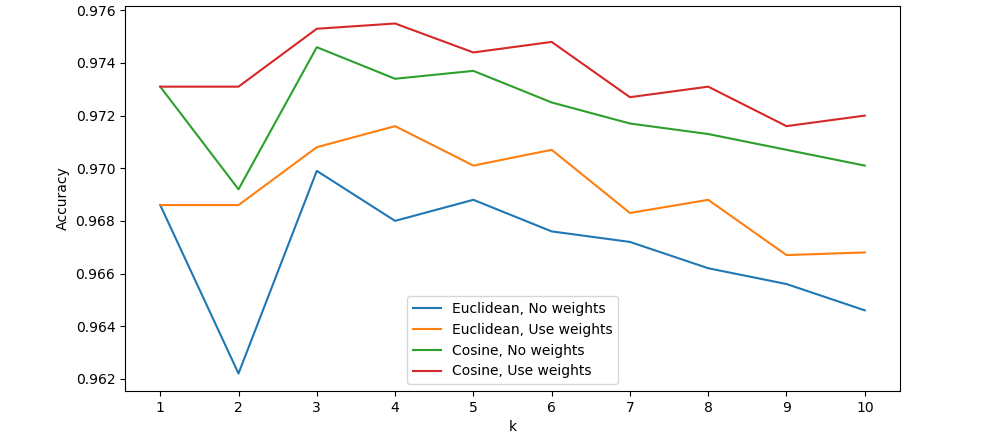
\includegraphics[scale=0.9]{\detokenize{./../experiment_2_3/scores_plot.png}}
%	\centering
%	\caption{Точность на тестовой выборке в зависимости от числа соседей, метрики и функции взвешивания}
%	\label{pic:1}
%\end{figure}

%\begin{table}[H]
%	\begin{tabular}{llll}
%		Euclidean; No weights & Euclidean; Use weights & Cosine; No weights & Cosine; Use weights \\
%		\hline
%		$199.60$                & $193.57$                 & $413.96$             & $\bm{414.58}$             
%	\end{tabular}
%	\caption{Время работы алгоритмов в зависимости от используемой метрики и функции взвешивания. Замер производился на кросс валидации с 3 фолдами.}
%	\label{tbl:2}
%\end{table}
	
	
\begin{section}{Введение}
	В данном отчёте описаны  эксперименты, направленные на изучение качества и скорости работы линейных алгоритмов классификации, а именно бинарной классификации (логистическая регрессия) и различных видов многоклассовой классификации (мультиномиальная классификация, подходы один-против-всех и каждый-против-каждого)\par
	Все эксперименты проведены на отзывах из датасета 20newsgroups ( - размер обучающей выборки, - размер тестовой выборки).
\end{section}

\begin{section}{Эксперименты}
	
\begin{subsection}{Логистическая регрессия}
	В данном разделе будут рассмотрены эксперименты с подвыборкой из исходного датасета, а именно положительные и отрицательные отзывы. Будут рассмотренны методы градиентного спуска (GD) и стохастического градиентного спуска (SDG). Также будет произведёт анализ влияния гиперпараметров на точность и скорость сходимости этих методов.
	
\begin{subsubsection}{Теоритические обоснования}
	Для реализации GD и SGD необходимо определить направление наискорейшего убывания функции потерь. В данном методе функция потерь имеет вид:
	$$ \mathbb{L} = -\frac{1}{N} \sum_{i=1}^{N} \ln(1 + \exp(-y_{i}x_{i}w)) + \frac{\lambda}{2}||w||_{2}^{2} $$
	Где $w \in \mathbb{R}^{d}$ - вектор столбец параметров, $x \in \mathbb{R}^{N*d}$ - множество объектов признаков, $y \in \{-1, 1\}^{N}$ - множество меток классов.
	Несложно убедиться, что:
	$$ \nabla{\mathbb{L}}_{w} = \frac{1}{N} \sum_{i=1}^{N} y_{i}x_{i}\frac{\exp(-y_{i}x_{i}w)}{1 + \exp(-y_{i}x_{i}w)} + \lambda w$$
\end{subsubsection}

\begin{subsubsection}{Градиентный спуск}
	В качестве гиперпараметров данного алгоритма рассматриваются параметры определяющие величину шага $lr = \frac{\alpha}{\beta^{n_{iter}}}$, где $n_{iter}$ - номер текущей эпохи. Были произведены замеры функции потерь и точности на обучающей и тестовой выборках в зависимости от номера итерации при различных значениях параметров $\alpha, \beta$:
\begin{figure}[H]
		\hspace*{-1.5cm}
	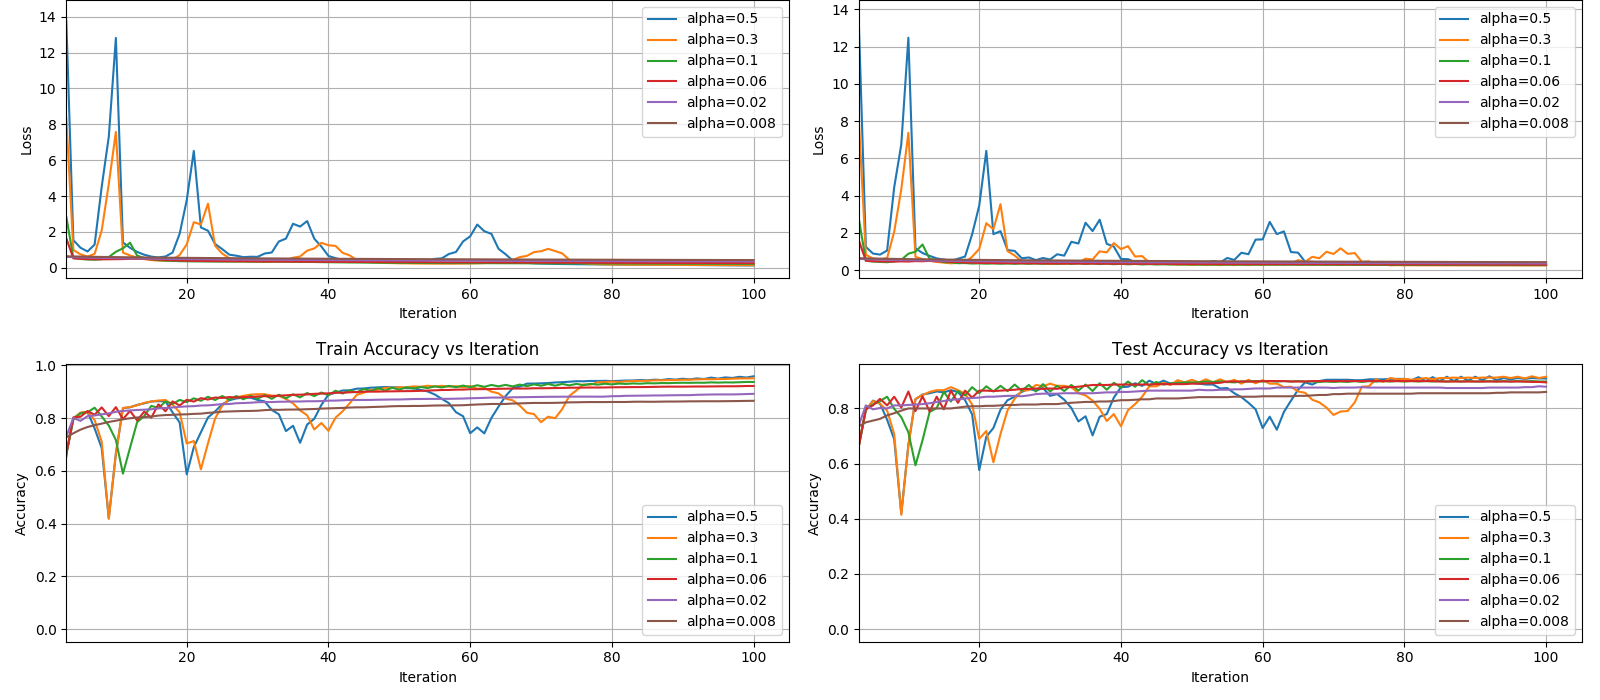
\includegraphics[scale=0.5]{\detokenize{./Plots/GDClassifier_alpha.png}}
	\centering
	\caption{Точность и функция потерь в зависимости от числа итераций при различных значениях $\alpha$. (При $\beta=0$)}
	\label{pic:1}
\end{figure}
	Из \ref{pic:1} можно видеть, что с уменьшением $\alpha$ сходимость метода на начальных итерациях улучшается и графики функции потерь и точности имеют меньшую дисперсию. В тоже время, с увеличением числа итераций данный эффект нивелируется за счёт стремления нормы градиента к $0$. Однако, более высокие значения $\alpha$ показывают лучшие результаты при большом числе эпох.
\begin{figure}[H]
	\hspace*{-1.5cm}
	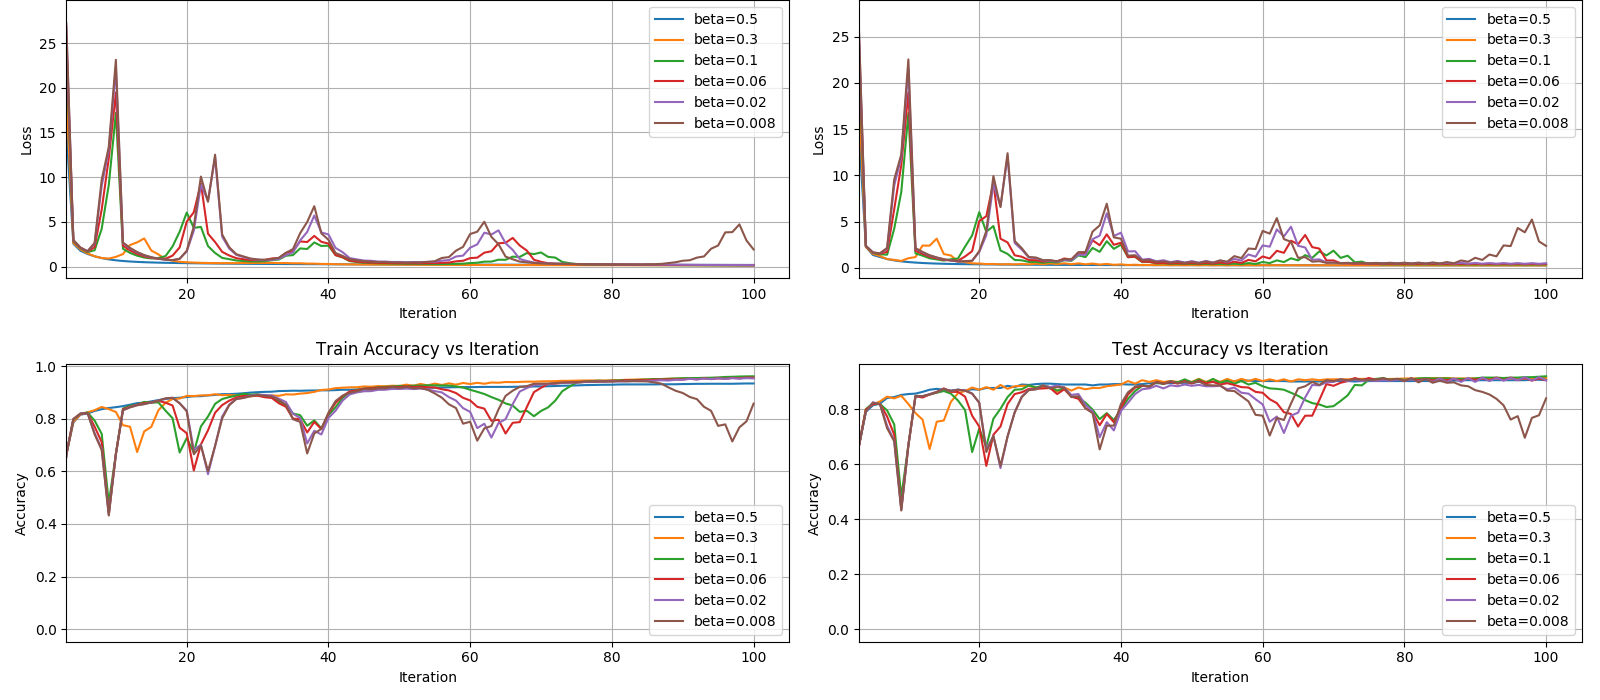
\includegraphics[scale=0.5]{\detokenize{./Plots/GDClassifier_beta.png}}
	\centering
	\caption{Точность и функция потерь в зависимости от числа итераций при различных значениях $\beta$. (При $\alpha=1$)}
	\label{pic:2}
\end{figure}
	Как можно видеть на рисунке \ref{pic:2} поведение графиков в зависимости от $\beta$ схоже с зависимостью от $\alpha$ - большие значения $\beta$ приводят к значительной амплитуде колебаний на начальных итерациях, но с ростом их числа, функция потерь и точность не только достигают тех же значений, что при малых $\beta$, но и незначительно их превосходят.

\end{subsubsection}
	Как известно, стохастический градиентный спуск позволяет не только увеличить скорость работы алгоритмов, но и привести к лучшим результатам как относительно точности, так и функции потерь. Сравним градиентный спуск, описанный в предыдущем разделе со стохастическим градиентным спускам в зависимости от тех же гиперпараметров. Так же исследуем реальное время работы алгоритма и его точность в зависимости от различных значений размера батча.
\begin{subsubsection}{Стохастический градиентный спуск}
	
\begin{figure}[H]
	\hspace*{-1.5cm}
	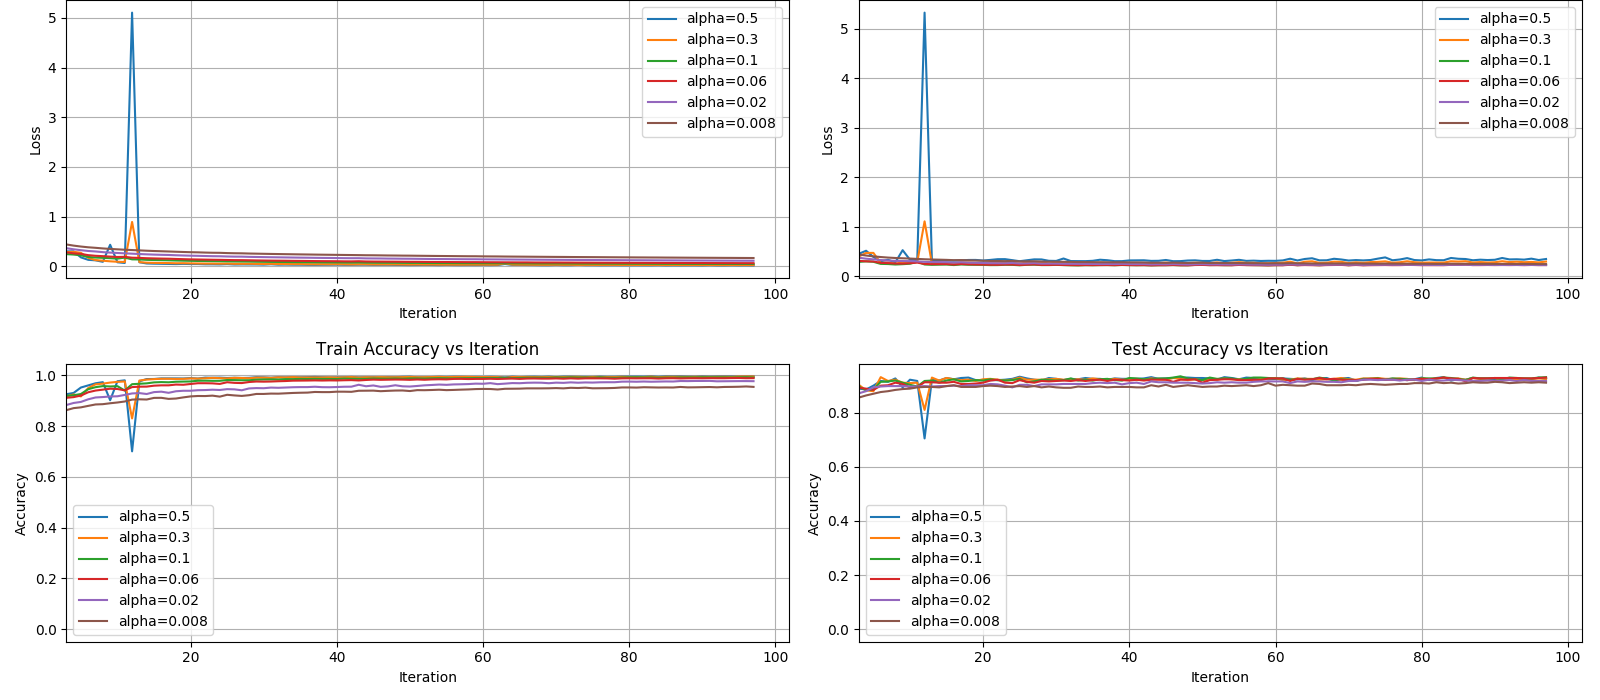
\includegraphics[scale=0.5]{\detokenize{./Plots/SGDClassifier_alpha.png}}
	\centering
	\caption{Точность и функция потерь в зависимости от числа итераций при различных значениях $\alpha$. (При $\beta=0$)}
	\label{pic:3}
\end{figure}

\begin{figure}[H]
	\hspace*{-1.5cm}
	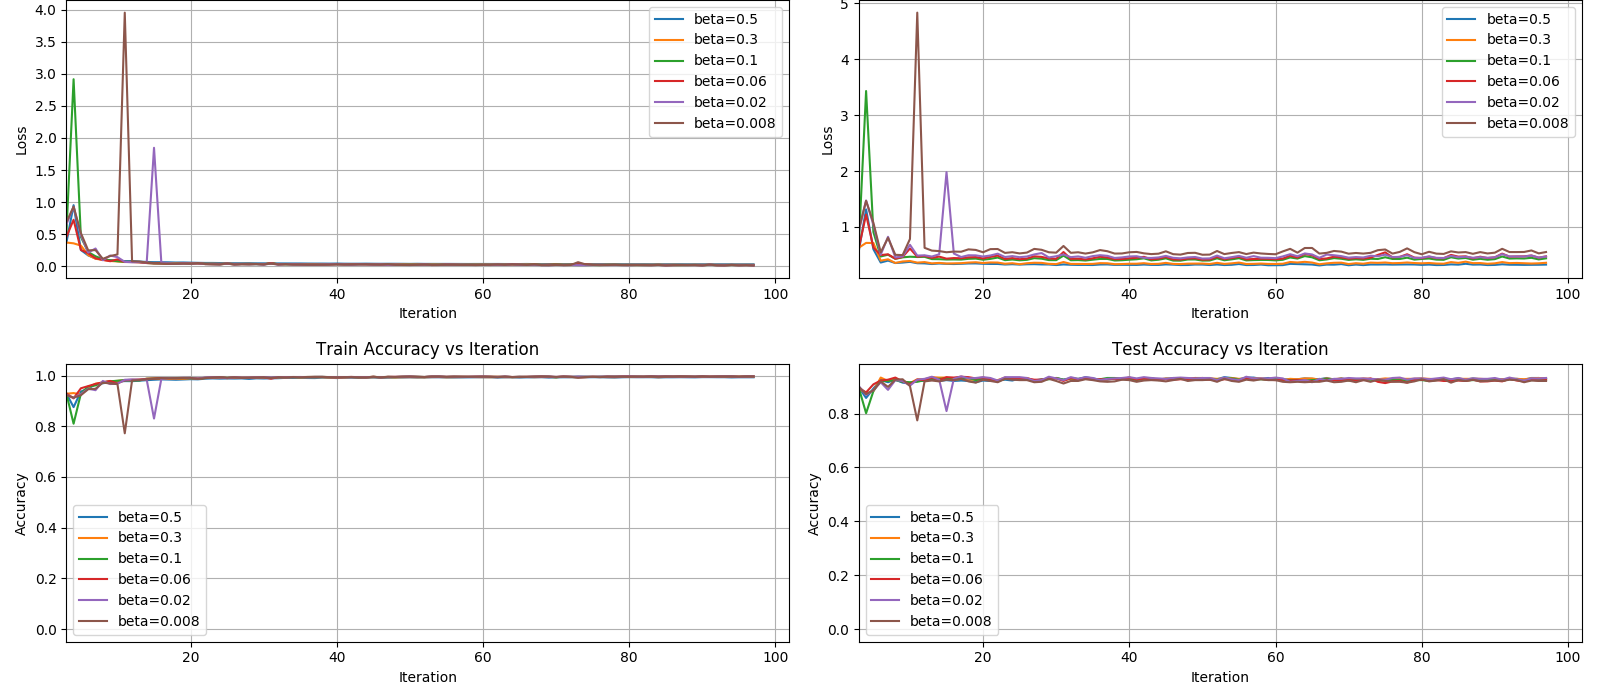
\includegraphics[scale=0.5]{\detokenize{./Plots/SGDClassifier_beta.png}}
	\centering
	\caption{Точность и функция потерь в зависимости от числа итераций при различных значениях $\beta$. (При $\alpha=1$)}
	\label{pic:4}
\end{figure}
	Как можно видеть из рисунков \ref{pic:3}, \ref{pic:4}, стохастический градиентый спуск позволяет методу более стабильно сходится в широком диапазоне значений $\alpha, \beta$. Таким образом, SGD намного проще обучать за счёт более простого подбора гиперпараметров. Сравним точность и значения функции потерь для GD и SGD при одних и тех же значениях гиперпараметров:
	\begin{figure}[H]
		\hspace*{-1.5cm}
		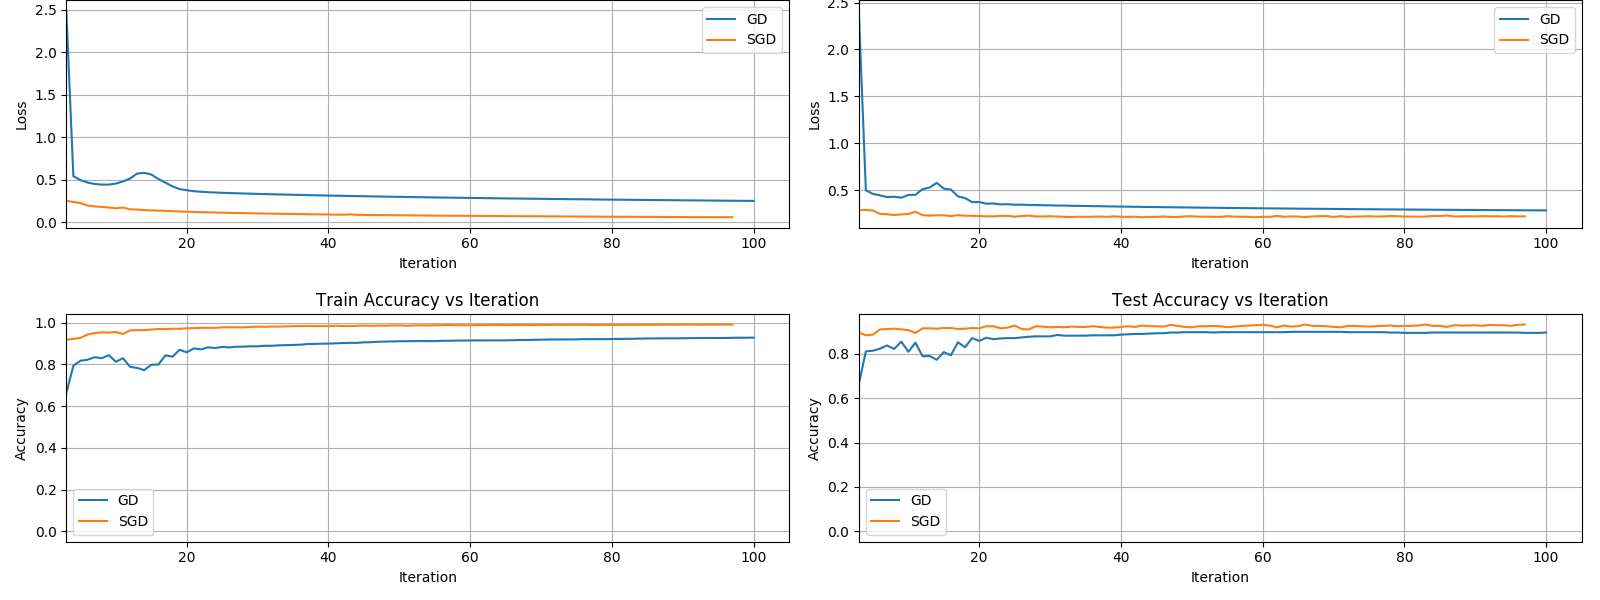
\includegraphics[scale=0.5]{\detokenize{./Plots/GD_vs_SGD.png}}
		\centering
		\caption{Точность и функция потерь в зависимости от числа итераций для GD и SGD}
		\label{pic:5}
	\end{figure}
	Можно видеть, что SGD превосходит GD как по точности, так и по значениям функции потерь.
	\par
	В конце, была исследована зависимость работы алгоритма в зависимости от размера батча:
	\begin{figure}[H]
		\hspace*{-1.5cm}
		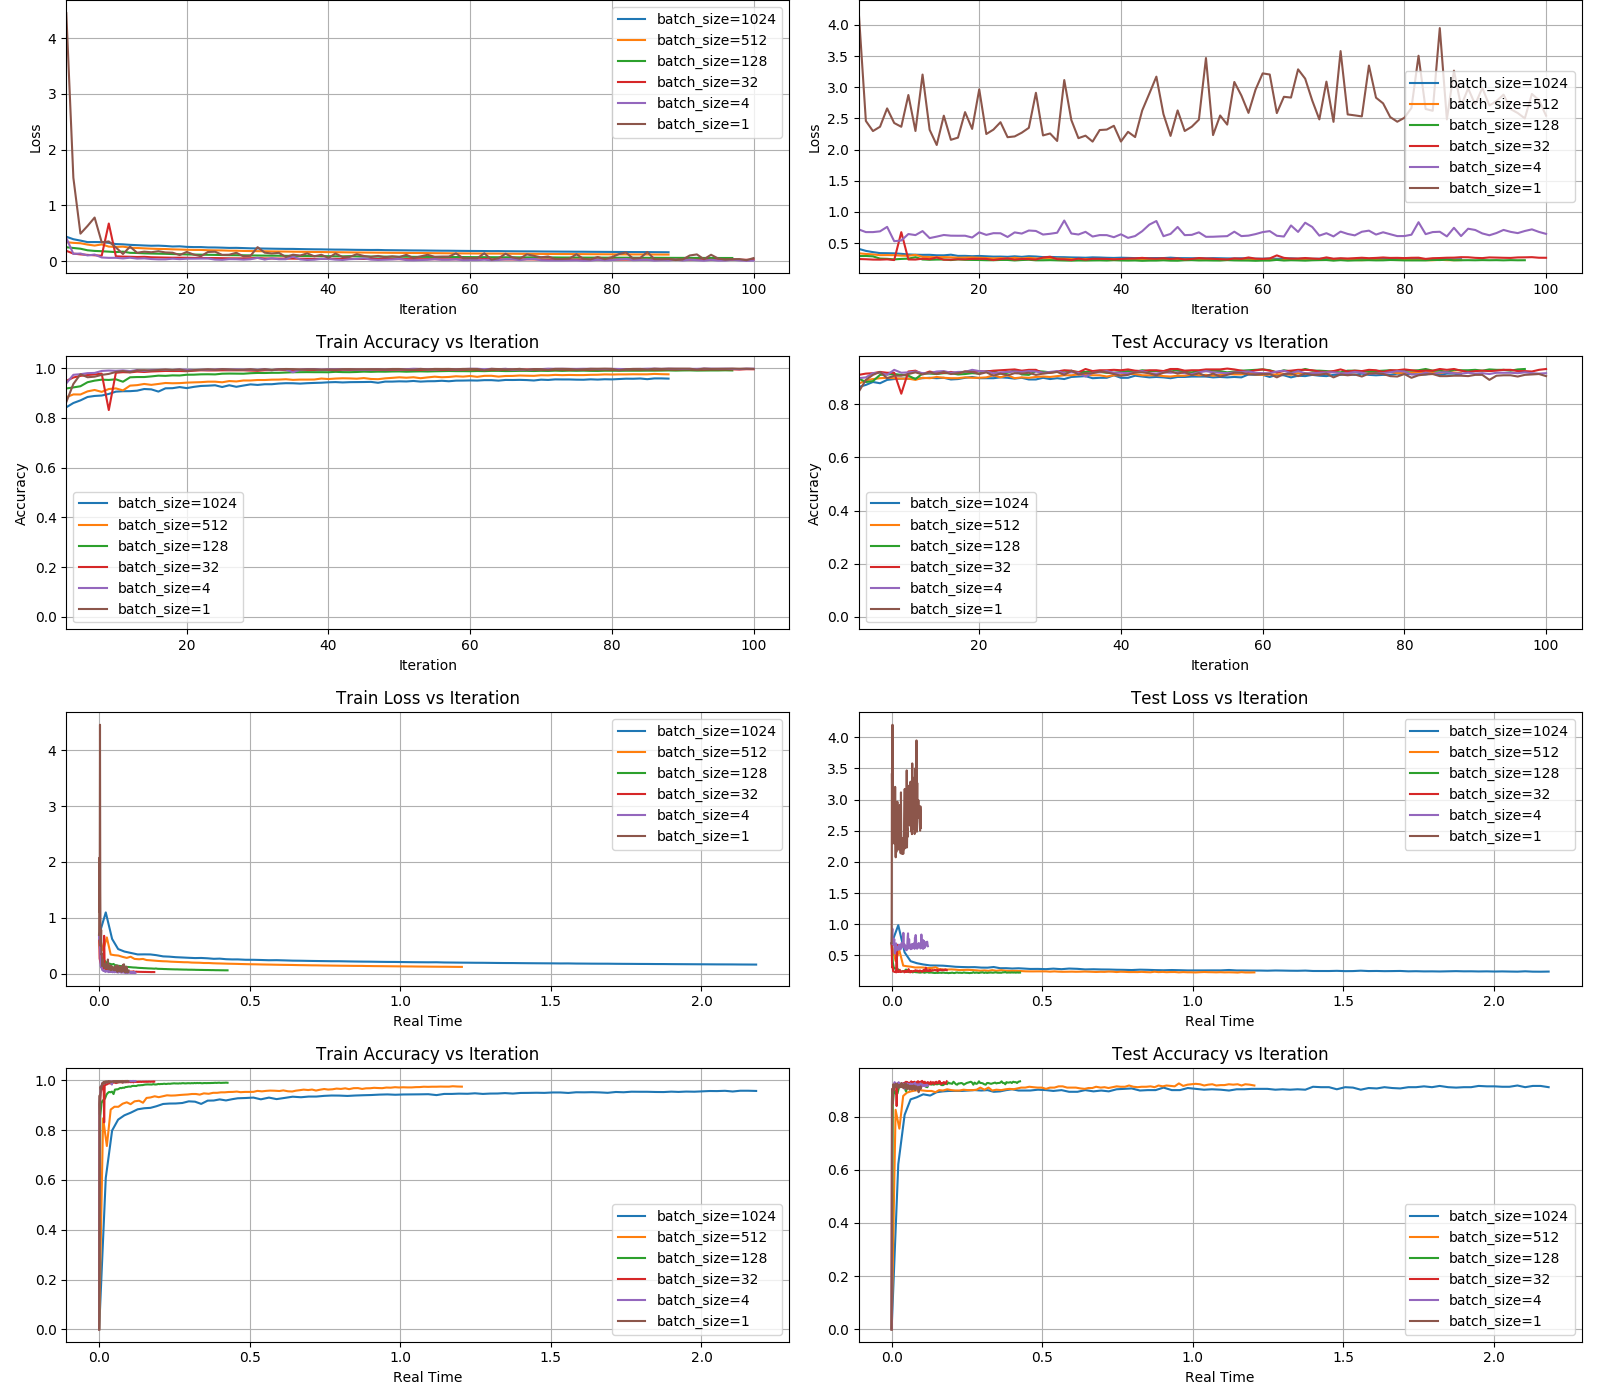
\includegraphics[scale=0.5]{\detokenize{./Plots/SGDClassifier_batch_size.png}}
		\centering
		\caption{Точность и функция потерь в зависимости от числа итераций при различных размерах батча ($\alpha=0.1, \beta=0.1$)}
		\label{pic:6}
	\end{figure}
	Из рисунка \ref{pic:6} видно несколько зависимостей:
	\begin{enumerate}
		\item Чем больше размер батча, тем дольше времени требуется, чтобы сделать одно и тоже число итераций
		\item Слишком маленькие размеры батча обучаются намного хуже, чем умеренные или большие размеры
		\item Начиная с размера батча $32$ нет существенной разницы в качестве работы алгоритмов.
	\end{enumerate}
\end{subsubsection}

\begin{subsubsection}{Выводы}
	В качестве результата, можно выделить, что SDG сходится стабильнее, быстрее и, в пределе, к лучшему результату нежели SD.
\end{subsubsection}

\end{subsection}

\begin{subsection}{Многоклассовая классификация}
		В данном разделе будут проведены эксперименты с исходным датасетом. Будут проведено сравнение мультиномиальной регрессии и методов один-против-всех, каждый-против-каждого. Также будет произведёт анализ влияния гиперпараметров на точность и скорость сходимости этих методов.
	
\begin{subsubsection}{Теоритические обоснования}
		Аналогично предыдущему пункту запишем функцию потерь в тех же обозначениях, за исключением того, что $w \in \mathbb{R}^{d*C}$ - матрица признаков:
		$$ \mathbb{L} = -\frac{1}{N} \sum_{i=1}^{N} x_{i}w_{y_{i}} + \frac{1}{N} \sum_{i=1}^{N} \ln(\sum_{k=1}^{C}\exp(x_{i}w_{k})) + \frac{\lambda}{2}||w||_{2}^{2} $$
		Дифференцируя функцию потерь поэлементно, получим:
		$$\frac{\partial\mathbb{L}}{\partial w_{jp}} = -\frac{I}{N}\sum_{i=1}^{N}x_{ip}[\mathbb{I}[j=y_{i}] - \mathbb{P}(y_{i}=j|x_{i})] + \lambda w_{jp}$$
		$$
		\mathbb{P}(y_{i}=j|x_{i}) = \frac{ \exp(x_{i}w^{j}) } {\sum_{k=1}^{C} \exp(x_{i}w^{k})}
		$$
		Подставляя $C = 2$ несложно убедиться, что данная формула переходит в аналогичную для логистической регрессии.
\end{subsubsection}
	
	
\begin{subsubsection}{Выбор оптимального алгоритма}
	В данной секции будет произведено сравнение трёх вышеназванных методов с целью выбора оптимального для дальнейших экспериментов.
	Для методов один-против-всех и каждый-против-каждого в качестве базового алгоритма используется SGD с параметрами $\alpha=0.1, \beta=0.1$ с максимальным числом итераций $100$ и размером батча $128$. Для мультиномиальной регрессии так же используется SGD c теми же гиперпараметрами, но число итераций ограничено $10$ ввиду значительно более медленной скорости работы алгоритма. Так же, экспериментальным путём обнаружено, что MN работает лучше всего при размере батча $1$, поэтому именно он будет использоваться в дальнейшем.
\begin{table}[H]
	\begin{tabular}{l|lll}
		- & One-vs-All & All-vs-All & MN \\
		 \hline
		Accuracy (Train/Test) & $0.722/0.665$ & $0.652/0.606$ & $0.666/0.621$ \\
	\end{tabular}
	\centering
	\caption{Точность для различных алгоритмов мультиклассовой классификации}
	\label{tbl:1}
\end{table}
	Для улучшения работы алгоритма была применена лемматизация (пакет pymystem) и удаление стоп-слов. 
\begin{table}[H]
	\begin{tabular}{l|lll}
		- & One-vs-All & All-vs-All & MN \\
		\hline
		Accuracy (Train/Test) & $0.722/0.665$ & $0.652/0.606$ & $0.772/0.697$ \\
	\end{tabular}
	\centering
	\caption{Точность для различных алгоритмов мультиклассовой классификации после лемматизации и удаления стоп-слов}
	\label{tbl:2}
\end{table}
Несмотря на то, что качество увеличилось, время работы алгоритма значительно возросло за счёт длительного времени предобработки данных (более 5 минут). Однако если сохранять предобработанные данне на диск между экспериментами, то можно нивелировать это время, и, более того, за счёт уменьшения размерности признакого пространства с $89000$ до $40000$.
\par
Ещё одним методом улучшения качества может служить использование более сложных признаков, чем BagOfWords, например, Tfidf.
\begin{table}[H]
	\begin{tabular}{l|lll}
		- & One-vs-All & All-vs-All & MN \\
		\hline
		Accuracy (Train/Test) $mindf=2$ & $0.498/0.498$ & $0.532/0.532$ & $0.775/0.705$ \\
		Accuracy (Train/Test) $mindf=4$ & $0.487/0.485$ & $0.522/0.519$ & $0.775/0.706$ \\
		Accuracy (Train/Test) $mindf=4$ & $0.487/0.486$ & $0.521/0.520$ & $0.773/0.708$ \\
	\end{tabular}	
	\centering
	\caption{Точность для различных алгоритмов мультиклассовой классификации после лемматизации, удаления стоп-слов с использованием Tfidf}
	\label{tbl:3}
\end{table}
Однако, как видно из таблицы \ref{tbl:3}, что данное изменение приводит к значительному падению качества в случае методов одни-против-всех и каждый-против-каждого. При этом для MN наблюдается значительный прирост качества.
\par
\end{subsubsection}

\begin{subsubsection}{Итоги}
	Можно отметить, что MN работает значительно лучше остальных алгоритмов даже с учётом небольшого числа итераций SGD. Как следствие, для итогового тестирования используются следующая модель: MN, обучаемая с помощью SGD ($\alpha=0.1, \beta=0.1$, размер батча $1$). Все данные предварительно лемматизированы и из них удалены стоп слова. Затем, выделены признаки Tfidf. В итоге был получен результат $0.891/0.772$ - точность на обучающей и тестовой выборке соответственно. При этом параметр $mindf$ почти не влияет на итоговый результат, что позволяет снизить размер признакового пространства до $10000$ без потери качества, но с увеличением скорости на порядок.	
	\par
	Изучая объекты, на которых алгоритм допускает ошибки можно выделить следующие особенности:
	\begin{enumerate}
		\item Маленькая длина отзыва
		\item Большое число спецсимволов и цифр
	\end{enumerate}
	
\end{subsubsection}

\end{subsection}

\end{section}

\begin{section}{Выводы}
	Эксперименты, проведённые в этом отчёте показывают, что:
	\begin{enumerate}
		\item SGD работает стабильнее, менее чувствителен к выбору гиперпараметров, имеет более высокую скорость сходимости.
		\item В целом, методы один-против-всех и каждый-против-каждого работают намного хуже MN. При этом, при снижении размерности признакового пространства, происходит значительное падение качества этих двух методов.
	\end{enumerate}
\end{section}

\end{document}